\documentclass[12pt,letterpaper,boxed]{hmcpset}
\usepackage[margin=1in,headheight=14pt]{geometry}
\usepackage{amsfonts, amsmath, amssymb, enumerate, fancyhdr, gensymb, lastpage, mathtools, parskip, graphicx}
\usepackage{xcolor, tikz-cd}
\newcommand{\wg}[1]{\textcolor{violet}{#1}}
\newcommand{\OO}{\mathcal O}
\newcommand{\Q}{\mathbb Q}
\newcommand{\R}{\mathbb R}
\newcommand{\C}{\mathcal C}
\newcommand{\Z}{\mathbb Z}
\newcommand{\abs}[1]{\left|#1\right|}
\newcommand{\im}{\text{im }}
\newcommand{\inv}{^{-1}}
\newcommand{\normal}{\unlhd} %% one can also use \trianglelelefteq
\newcommand{\anglee}[1]{\langle #1 \rangle}
\usepackage[shortlabels]{enumitem}

% Numbering macros
\pagestyle{fancy}
\lhead{Will Gilroy}
\chead{Algs Homework \#}
\rhead{03 November 2021}
\lfoot{}
\cfoot{}
\rfoot{Page\ \thepage\ of\ \pageref{LastPage}}

\linespread{1.5}

\newcommand\blankpage{
    \thispagestyle{empty}
    \addtocounter{page}{-1}
    \newpage}
\renewcommand\footrulewidth{0.4pt}

\begin{document}

\problemlist{Algorithms HW } 

%------------------------- Problem 1 -----------------------

\begin{problem}[1]
	\hfill
\end{problem}

\begin{solution}
\end{solution}

\newpage

%------------------------- Problem 2 -----------------------

\begin{problem}[2]
	\hfill
\end{problem}

\begin{solution}
\end{solution}

\newpage

%------------------------- Problem 3 -----------------------

\begin{problem}
	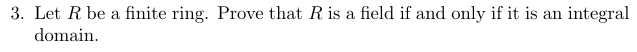
\includegraphics[scale=0.8]{3.png}
	\hfill
\end{problem}
\begin{solution}
In general we have that $R$ a field implies $R$ is an integral domain,
even if $R$ is not finite. We recount the proof here.
Suppose $R$ is a field, that is $R$ is commutative with $1 \neq 0$ and
every $a \in R$ is a two-sided unit. Now suppose we have $ab = 0$.
If $a = 0$ then we are done, so suppose 
$a$ is non-zero in
$R$. Then, $a$ has a two-sided inverse $a\inv \in R$, and so \[
	0 = ab = a\inv a b = 1 \cdot b = b.
\]
If we instead assume $b \neq 0$ then 
an extremely similar calculation will show that $ab = 0$ implies $a =
0$. \wg{(Or, perhaps it's enough that $R$ is commutative at this
point?)} 
Thus, $R$ is an integral domain.

Now suppose $R$ is finite and is an integral domain. That is, $R$ is a
commutative ring with $1 \neq 0$ and for all $a,b \in R$ we have $ab =
0$ implies $a = 0$ or $b = 0$. We show that every non-zero element in
$R$ has a two-sided inverse.
Let $a \in R$ be some non-zero element and let $\phi_a: R \to R$ be
the map defined by $\phi(r) = a\cdot r$. 

We claim that $\phi_a$ is
injective. Suppose we have $\phi(b) = \phi(c)$ for some $b,c \in R$.
That is, $ab = ac$, equivalently $a(b-c)= 0$. But recall that $a$ is a
non-zero element in the integral domain $R$, and so we must have $b-c = 0$. In
other words $b = c$ and $\phi_a$ is injective by definition.

In addition, since $R$ is finite and $\# R = \# R$, we have that
$\phi_a$ is actually a bijection. And so there must exist some $c \in
R$ such that $\phi(c) = 1$. That is, we have $c \in R$ such that $a c
= 1$. Since $R$ is commutative, $a$ is actually a two-sided unit with
inverse $c$. Thus, $R$ is a field.

\wg{Note to self: Aluffi claims that finite division rings turn out to
always be commutative. Have a read of this later if we get time}
\end{solution}

\newpage

%------------------------- Problem 4 -----------------------

\begin{problem}
	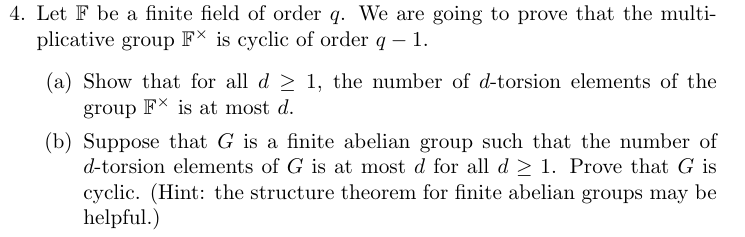
\includegraphics[scale=0.8]{4.png}
	\hfill
\end{problem}

\begin{solution}

\begin{enumerate}[(a)]
\item Consider the polynomial $f(x) = x^n - 1 \in \mathbb F[x]$. 
Recall that $\mathbb F[x]$ is a unique factorization domain
\wg{we should probably understand this better}, and so $f$ has at most
$n$ roots in $\mathbb F$. That is, there are at most $n$ elements in
$\mathbb F$ such that $a^n = 1$. And, in particular, the zero element
in the ring $\mathbb F$ does not satisfy the above equation. And so,
all roots of $f$ must in fact lie in $\mathbb F^\times$. 
Then, recalling that an element in a group $g \in G$ is a $d$-torsion
element of $G$ if $\abs g \,\vert \, d$, the above shows that $\mathbb
F^\times$ has at most $d$ elements with $d$-torsion, for each $d \geq
1$. 
\wg{question: does $d$-torsion mean that $\abs g = d$ or that $\abs g \vert d$?}


\item I'm not sure we've super talked about the structure theorem of
finite abelian groups much, so I will recall the theorem in detail
here. \textit{Theorem:} If $G$ is a finite abelian group then we have
that $G$ is a product of cyclic groups, in particular
\[
	G \cong \Z / d_1 \Z \oplus \cdots \oplus \Z /d_s \Z,
\]
for $d_i > 0$ integers and where $d_1 \, \vert \, d_2 \vert \cdots \vert
d_n$ \wg{ew, i hate the spacing on this}. Moreover, $\abs G = d_1
\cdots d_s$. Here, we are treating $G$
as a group under addition. 

Now suppose $G$ is a finite abelian group such that the number of
$d$-torsion elements is at most $d$ for all $d \geq 1$. We show that
$s = 1$ and so $G$ is cyclic. Suppose, for contradiction,
that $s > 1$ and let $g \in G$.
We have that $\anglee g \leq G$ and so, by Lagrange's theorem, we have
that $\abs g \vert \abs G = d_1 \cdots d_s$. And so $\abs g$ divides
one of $d_i$. If $\anglee g$ divides $d_i$ then, since in particular
$d_i \vert d_s$, we also have $\anglee g \vert d_s$.
Indeed, we have $m_1 \abs g = d_i$ and $m_2 d_i = d_s$ then $m_1m_2
\abs g = d_s$, i.e., $\abs g \vert d_s$. That is $g$ is a
$d_s$-torsion element.

We have shown that all elements $g \in G$ have $d_s$-torsion.
However, we have $\abs G = d_1 \cdots d_s > d_s$. And
so we have found more than $d_s$ elements of $G$ which have
$d_s$-torsion, a contradiction. That is, we must in fact have $s=1$
and $G \cong
\Z/d\Z$ for some $d \in \mathbb N$. In other words, $G$ is a cyclic
group.


\end{enumerate}
\end{solution}

\newpage
%------------------------- Problem 5 -----------------------

\begin{problem}
	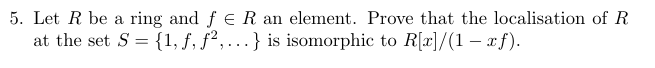
\includegraphics[scale=0.8]{5.png}
	\hfill
\end{problem}

\begin{solution}
Let us first define a map into $R[x]$: $\phi: S\inv R \to R[x]$ by 
$\varphi(1/f) = x$ and $\phi(a/1) = a$, and then we extend this
definition so that the map distributes over products and addition in
$S\inv R$. That is $\phi(a/f^k) = ax^k$ and $\phi(a/f^k + b/f^\ell) =
\phi((af^\ell + b^k)/f^{k+\ell}) = (af^k + bf^\ell)x^{k+\ell}$. 
\wg{Is this sufficient reasoning to allow us to ``extend the map''}.

First we check that this is a well defined map out of $S\inv R$. 
Suppose $a/f^k \equiv b/f^\ell$ and consider
\[
	\phi(a/f^k - b/f^\ell) = \phi(\frac{af^\ell - bf^k}{f^{\ell+k}})
		= (af^\ell - bf^k)x^{\ell+k}.
\]
Now, the condition $a/f^k \equiv b/f^\ell$ means that there exists
some $c \in S$ such that $c(af^\ell - bf^k) = 0$, in particular $c =
f^m$ for some integer $m \geq 0$. That is, we have $f^m(af^\ell -
bf^k) = 0$. Applying $\phi$ to both sides of this expression gives
$x^m(af^\ell - bf^k) = 0$ in $R[x]$. \wg{If we somehow knew that $\ell
+ k \geq m$ we'd be done, but it's not super clear to me how we can
finish this reasoning. This might also perhaps be the wrong approach}

\wg{Actually note that $\phi: S\inv R \to R[x]$ is not a well-defined
map, consider the image of $(af^2)/f^3$}

Next we check that $\phi$ is in fact a well-defined map into the
quotient $R[x]/(1-fx)$. Namely, we will check that $\phi\inv((1-fx)) =
\{0\}$. We have \[
	\phi\inv(1-fx) = \frac{1}{1} - \frac{f}{f} = 0 \in S\inv R. 
\]
And so, $\phi$ is a well-defined map into the quotient $R[x]/(1-fx)$.
From now, we will treat $\phi$ as a map $\phi: S\inv \to R[x]/(1-fx)$.
\wg{Something about this paragraph feels a bit fishy to me, do we
think that I checked everythign that I needed to check?}

Nex we will show that $\phi$ is a bijection. First we check
injectivity. Notice that every element of $S\inv R$ can be reduced to
the form $a/f^k$ for some $a \in R$ and some natural $k$. Now suppose
$\phi(a/f^k) = \phi(b/f^\ell)$, i.e. $ax^k = bx^\ell$. The only way
for this to be true is if $k = \ell$ and only if $a = b$ \wg{a part of
me wants to unpack this, I believe this is true because intuitively
``the constants in $R[x]$ are independent of the variable $x$.'' is
there a more precise way of saying this?}.
That is, $a/f^k = b/f^\ell$ and so $\phi$ is injective.

Next we show that $\phi$ is surjective. Suppose
$a_0 + a_1x + \cdots a_nx^n \in R[x]/(1-fx)$, since this is an element
of the quotient suppose we have reduced away all existing factors of
$f$ in each coefficient $a_i$ using the relation $1 = fx$ in the
quotient.
Then notice $a_0/1 +
a_1/f + \cdots a_n/f^n$ maps to the given polynomial under $\phi$.

In the end, we have found a bijective homomorphism from $S\inv R$ to
$R[x]/(1-fx)$, and so these rings are isomorphic. 
\end{solution}

\newpage
%------------------------- Problem 6 -----------------------

\begin{problem}[4]
	\hfill
\end{problem}

\begin{solution}
\end{solution}

\newpage

%------------------------- Problem 7 -----------------------

\begin{problem}[4]
	\hfill
\end{problem}

\begin{solution}
\end{solution}

\newpage

%------------------------- Problem 8 -----------------------

\begin{problem}[4]
	\hfill
\end{problem}

\begin{solution}
\end{solution}

\newpage



\end{document}
